\paragraph{}En esta página se puede observar el listado completo de todos los microcontroladores existentes en el catálogo electronico y además. En la parte derecha de la especificación de cada microcontrolador, se halla el botón para añadir dicho microcontrolador al carrito de la compra, actualizando además dinámicamente el número de ítems en el icono del carro incrementándolo en uno.

\begin{figure}[h!]
	\centering
	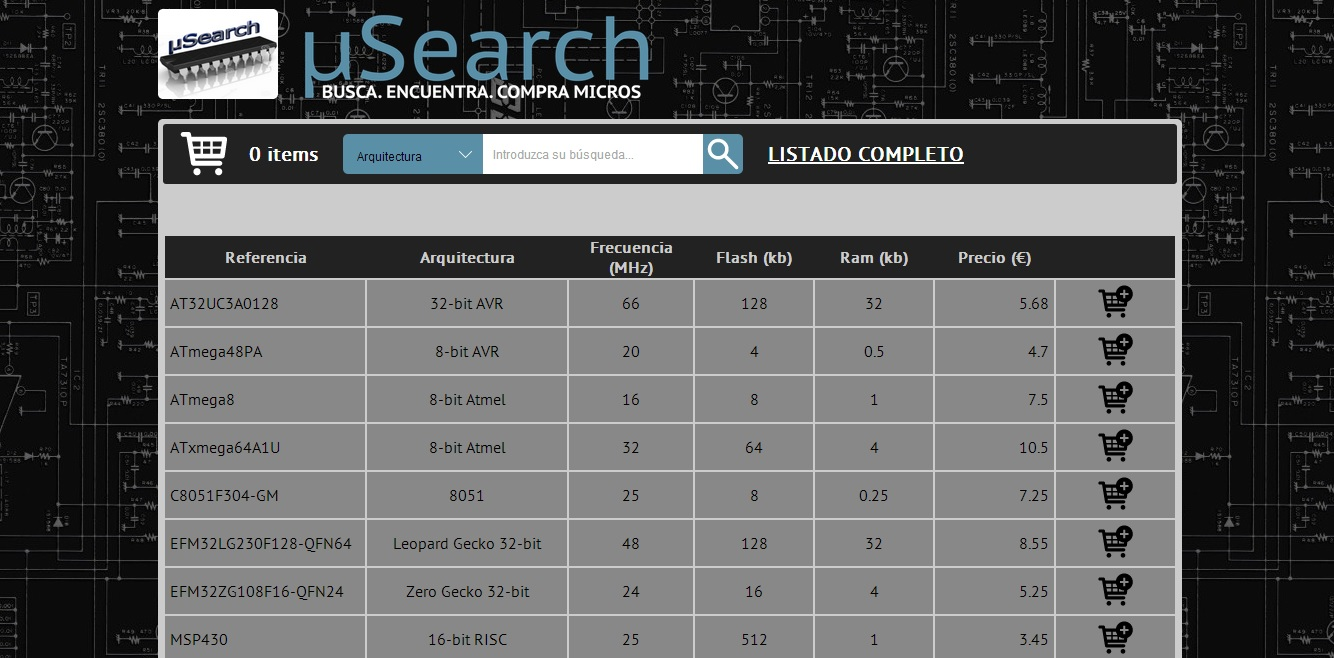
\includegraphics[width=0.85\textwidth]{img/listado_completo_user}
	\caption{Página de listado completo de micro-controladores.}
	\label{fig:listado_completo_user}
\end{figure}

Como en todas las demás páginas del sitio web, si se pulsa en cualquiera de los dos logotipos del catálogo $\mu$Search (esquina superior izquierda), el sistema redirigirá al usuario a la página inicial del catálogo.

\paragraph{}Desde esta página, a través de los iconos situados en la cabecera debajo de los logotipos de la web, el usuario puede acceder a:

\begin{itemize}
	\item\textbf{Carrito de la compra:} Pulsando sobre este botón el usuario será redirigido a la página del carrito de la compra.
		
	\item \textbf{Búsqueda:} Desde esta sección, el usuario puede realizar búsquedas sobre el catálogo de microcontroladores en base a cualquiera de las características de un microcontrolador (Arquitectura, Frecuencia, Flash, RAM). Simplemente se debe seleccionar una de las características de la lista despegable, introducir el texto a buscar y pulsar sobre el icono de búsqueda.
	El usuario será redirigido a una página donde se le mostrará el resultado de la búsqueda en forma de lista de microcontroladores.
		
	\item \textbf{Listado Completo:} Pulsando sobre este botón/icono se recargará la página actual.
\end{itemize}